\chapter{Implementation}
\label{ch:Implementation}

This chapter describes the theoretical design of the filter algorithm and its implementation, based on the fundamentals acquired in the previous chapters. Subsequently, the experiments and its results are presented.

\section{Initial Situation}

There were already a variety of Kalman filter algorithms implemented. They served as a reference, in tandem with an orientation estimation based on a Qualisys motion capture system using cameras in combination with optical markers. The placement of the markers on the leg are depicted in Figure \ref{fig:marker_placement}. From the recorded motion of the markers in space the motion capture system computed the orientation angles of the thighs and shanks.

(Any algorithms that are already implemented for comparison that I can cite or state and describe how they differ from the one that I will implement??)

\begin{figure}
\centering
	\begin{tikzpicture}[auto, thick, node distance=3cm,>=latex']
    \pgftext{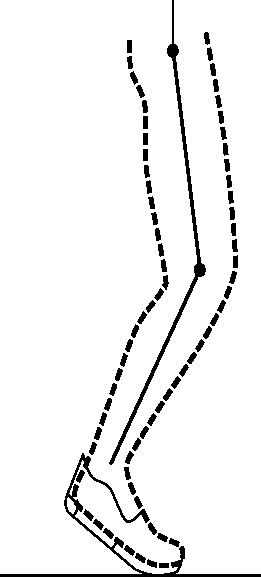
\includegraphics[width=3.5cm]{images/sensors_on_leg}} at (0pt,0pt);
    \node [] (a) at (-4.4, -2) {};
    \node [] (b) at (-4.5, 0.1) {};
    \node [] (c) at (4.45, 3.3) {};
\end{tikzpicture}
\caption{Human leg with optical markers, from \cite{tao_gait_2012}.} \label{fig:marker_placement}
\end{figure} 

\section{Theoretical Design}\label{sec:theoretical_design}

This section maps the theoretical design of the system proposed by \citeauthor{bennett_motion_2014} in \cite{bennett_motion_2014} to the existing GaitWatch system. It states the assigned coordinate frames and the conventions with respect to rotation about them. Furthermore, it describes the kinematic model and the extended Kalman filter in detail.

\subsection{Kinematic model}

The \emph{kinematic model} relates the respective angles of the thigh and shank about the hip and knee joint to the acceleration seen by the wearable sensors. When walking in a straight line, the human leg can be modelled as a two-link planar revolute robot \cite{bennett_motion_2014}. Then, thighs and shanks remain in a single plane which is approximately parallel to the direction of motion. As depicted in Figure \ref{fig:robot}, the revolute joints of the \gls{pendubot} represent the hip und knee joint, and the two links the thigh and shank, respectively. The origin of the inertial world frame is located at the base of link 1, the upper of both links. The $x$-axis points forward, the $y$-axis points out from the hip to the right, and the $z$-axis points down. Thus, since the figure depicts the right leg from lateral, the $y$-axis points out of the page. This configuration follows the right-hand rule, which can also be used to determine the sense of rotation around the axes. The angle $\theta_1$ is measured with respect to the $x$-axis, and the angle $\theta_2$ of link 2, with respect to link 1. 

\begin{figure}
\centering
\begin{tikzpicture}[auto, thick,>=latex']
	\node [draw, rectangle, minimum height=1.6cm, minimum width=1.6cm, pattern=north west lines] at (0,0) (solid) {};

    \node [draw,  fill=white, very thick, rectangle, rounded corners=3pt, minimum height=3.7cm, minimum width=1cm, align=center, rotate around={30:(0,0)}] at (0.7, -1.25) (link1) {};
    \node [draw, thick, fill=gray, rounded corners=2pt, rectangle, minimum height=0.8cm, minimum width=0.5cm, align=center, rotate around={30:(0, 0)}, label={[label distance=0.18cm]335:IMU 1}] at (0.98, -1.7) (sensor1) {};
    
    \node [draw, fill=white, very thick, rectangle, rounded corners=3pt, minimum height=3.7cm, minimum width=0.6cm, align=center, rotate around={145:(0,0)}] at (0.6, -3.7) (link2) {};
    \node [draw, thick, fill=gray, rounded corners=2pt, rectangle, minimum height=0.8cm, minimum width=0.5cm, align=center, rotate around={145:(0, 0)}, label={right:IMU 2}] at (0, -4.56) (sensor2) {};
    
    \node[coordinate] (X) at (2.5,0) {};
    \node[coordinate] (Y) at (0,-2.5) {};
    \node[coordinate] (O) at (-0, 0) {};
    
    \draw[->] (O) -- node[name=x] {$x$}(X);
    \draw[->] (O) -- node[pos=0.6, name=y, label={left:$z$}] {}(Y);
    
    \draw[->] (0, -4.56) -- node[name=x_2] {$x_2$}(1.5, -5.6);
    \draw[->] (0, -4.56) -- node[name=x_2] {$z_2$}(-1.1, -6.1);
   
    \draw[dotted] (O) -- (2.5,-4.3);
    \draw[fill=white] (0,0) circle (4pt);
    \draw[fill=black] (0,0) circle (1pt) node[label={[label distance=-1.2mm]180:$y$}]{};
    \draw (1.45, -2.5) circle (4pt);
    
    \draw[-stealth] (1.2,-1) arc (300:355:1.2);
    \draw[-stealth] (0.8,-4.1) arc (240:303:1.4);
    
    \node at (1.3, -0.4) (angle1) {$\theta_1$};
    \node at (1.5, -3.7) (angle1) {$\theta_2$};
\end{tikzpicture}
\caption{Kinematic model of the human leg, from \cite{bennett_motion_2014}.} \label{fig:robot}
\end{figure} 

The \glspl{IMU} placed on the thighs and shanks measured the angular velocity and linear acceleration of the thighs and shanks, respectively. According to \citeauthor{spong2005robot} \cite{spong2005robot}, the $x$ and $z$ displacement and its derivatives in the world frame are as follows:

\begin{align}
  x &= a_1 \cos \theta_1 + a_2 \cos(\theta_1 + \theta_2) \\
  \dot{x} &= -a_1 \dot{\theta}_1 \sin \theta_1  - a_2 (\dot{\theta}_1 + \dot{\theta}_2) \sin(\theta_1 + \theta_2) \\
  \ddot{x} {}&= -a_1 [\dot{\theta}^2_1 \cos \theta_1 + \ddot{\theta}_1 \sin \theta_1] - a_2 [(\dot{\theta}_1 + \dot{\theta}_2)^2 \cos(\theta_1 + \theta_2) \nonumber \\ 
  &\mathrel{\phantom{=}} + (\ddot{\theta}_1 + \ddot{\theta}_2) \sin(\theta_1 + \theta_2)] \label{eq:acc_x} \\
  \nonumber \\
  z &= -a_1 \sin \theta_1 - a_2 \sin(\theta_1 + \theta_2) \\
  \dot{z} &= -a_1 \dot{\theta}_1 \cos \theta_1  - a_2 (\dot{\theta}_1 + \dot{\theta}_2) \cos(\theta_1 + \theta_2) \\
  \ddot{z} {}&= -a_1 [\ddot{\theta}_1 \cos \theta_1 - \dot{\theta}^2_1 \sin \theta_1] - a_2 [(\ddot{\theta}_1 + \ddot{\theta}_2) \cos(\theta_1 + \theta_2) \nonumber \\ 
  &\mathrel{\phantom{=}} + (\dot{\theta}_1 + \dot{\theta}_2)^2 \sin(\theta_1 + \theta_2)] \label{eq:acc_y}
\end{align}

\noindent
in which $a_1$ and $a_2$ are the lengths of the two links, respectively. Using Equations \ref{eq:acc_x} and \ref{eq:acc_y}, and the estimate of the angles $\theta_1$ and $\theta_2$ from the accelerometers we can 

The orientation of the sensor frames at rest are different from the world frame and dynamic when the pendulum is in motion. In order to transform the values from the world frame to the dynamic body frame of \gls{IMU} 2, which is seen in Figure \ref{fig:robot}, we used the transformation matrix $\mathbf{T}_y(\theta)$ from Equation \ref{eq:transformation_matrices} in transposed form. The positive sense of rotation according the right-hand rule is opposite to the mathematically positive sense, which is why we use the transpose of the transformation matrix. The body frame of sensor two is not aligned with the world frame for $\theta_1 = \theta_2 = 0$. Thus, an offset of $-\frac{\pi}{2}$ is necessary. With $\theta = \theta_1 + \theta_2 - \frac{\pi}{2}$, this yields

\begin{equation}
\mathbf{T}^T_y(\theta_1 + \theta_2 - \frac{\pi}{2}) = \begin{bmatrix}
    \cos (\theta_1 + \theta_2 - \frac{\pi}{2}) \; & 0 \; & \sin (\theta_1 + \theta_2 - \frac{\pi}{2}) \\
    0 \; & 1 \; & 0 \\
    -\sin (\theta_1 + \theta_2 - \frac{\pi}{2}) \; & 0 \; & \cos (\theta_1 + \theta_2 - \frac{\pi}{2})
    \end{bmatrix}\,.
\end{equation}

\noindent
The rotated tangential and radial components of the motion based acceleration estimates, $A_{rad}$ and $A_{tan}$ are found using the tranformation matrix to rotate the results of Equations \ref{eq:acc_x} and \ref{eq:acc_y}, respectively, according to Equation \ref{eq:transformation}.

\begin{equation}
  A_{rad} = \mathbf{T}^T_y(\theta_1 + \theta_2 - \frac{\pi}{2}) \ddot{x}
\end{equation}

\begin{equation}
  A_{tan} = \mathbf{T}^T_y(\theta_1 + \theta_2 - \frac{\pi}{2}) \ddot{z}
\end{equation}

Then, the tangential and radial acceleration estimates are subtracted from the sensor readings $A_x$ and $A_y$, which leaves an estimate of the gravity based acceleration $\mathbf{g}$ that acts on the sensor:

\begin{equation}
\mathbf{g} = \begin{bmatrix}
    g_x \\
    g_y 
    \end{bmatrix} = 
    \begin{bmatrix}
    A_x \\
    A_y 
    \end{bmatrix} -
    \begin{bmatrix}
    A_{rad} \\
    A_{tan} 
    \end{bmatrix}\,.
\end{equation}

\noindent
According to Equation \ref{eq:projection_gravity} the improved angle estimate is

\begin{equation}
  \theta = \mbox{atan}2(g_y, g_x)\,.
\end{equation}

\noindent
This angle can be used to reduce the estimation error due to gyroscope drift.

\subsection{Extended Kalman Filter Model}

The state-space model of the extended Kalman filter is given by the state vector

\begin{equation} \label{eq:state_vector}
  \mathbf{x} = \begin{bmatrix}
  	x, & z, & \theta_1, & \omega_1, & \alpha_1, & \theta_2, & \omega_2, & \alpha_2, & \beta_1, & \beta_2
  \end{bmatrix}^T
\end{equation}

where $x$ and $y$ correspond to the horizontal and vertical position of the end of link 2 with respect to the origin of the world frame, i.\,e. the hip joint. $\theta_1$ is the angle, $\omega_1$ the angular velocity, and $\alpha_1$ the angular acceleration of the first joint, respectively. The corresponding values for the second link are $\theta_2$, $\omega_2$, and $\alpha_2$. The biases from the gyroscope on the first and second sensor are $\beta_1$ and $\beta_2$, respectively. They are assumed to be constant or slowly time varying.

The measurement matrix $\mathbf{z}$ is given by

\begin{equation} \label{eq:measurement_vector}
  \mathbf{z} = \begin{bmatrix} z_1 \\ z_2 \\ z_3 \end{bmatrix} = \begin{bmatrix}
  	\omega_1 + \beta_1, & \omega_1 + \omega_2 + \beta_2, & \theta_1 + \theta_2
  \end{bmatrix}^T + \mathbf{v}\,.
\end{equation}
 
\noindent
where $\mathbf{v}$ is the random measurement noise process. The element $z_1$ represents the measurement of the first link angular velocity, which is the sum of the first link rotation and the gyroscope 1 bias. Equally, the element $z_2$ represents the measurement of the second link angular velocity, which is the sum of the first and second link rotation and the bias of gyroscope 2. Finally, the element $z_3$ is the angle estimate of the second accelerometer, which will see the angular displacement of both links.

As outlined in {20} the state equations at each iterations can be linearised as follow. The derivative of the state vector is

\begin{equation} \label{eq:state_vector_derivative}
  \dot{\mathbf{x}} = f(\mathbf{x}) = \left[\begin{smallmatrix}
  -a_1 [\dot{\theta}^2_1 \cos \theta_1 + \ddot{\theta}_1 \sin \theta_1] - a_2 [(\dot{\theta}_1 + \dot{\theta}_2)^2 \cos(\theta_1 + \theta_2) \\
  a_1 [\ddot{\theta}_1 \cos \theta_1 - \dot{\theta}^2_1 \sin \theta_1] + a_2 [(\ddot{\theta}_1 + \ddot{\theta}_2) \cos(\theta_1 + \theta_2) \\ \omega_1 \\ \alpha_1 \\ \omega_2 \\ 0 \\ 0 \\ 0 \\ 0 \\ 0
  \end{smallmatrix}\right]
\end{equation}

\noindent
This can be written as

\begin{equation}
  \dot{\mathbf{x}} = \mathbf{F} \mathbf{x}
\end{equation}

\noindent
with

\begin{equation}
\mathbf{F} = \begin{bmatrix}
  0 & 0 & 0 & A & 0 & 0 & B & 0 & 0 & 0\\
  0 & 0 & 0 & C & 0 & 0 & D & 0 & 0 & 0\\
  0 & 0 & 0 & 1 & 0 & 0 & 0 & 0 & 0 & 0\\
  0 & 0 & 0 & 0 & 1 & 0 & 0 & 0 & 0 & 0\\
  0 & 0 & 0 & 0 & 0 & 0 & 0 & 0 & 0 & 0\\
  0 & 0 & 0 & 0 & 0 & 0 & 1 & 0 & 0 & 0\\
  0 & 0 & 0 & 0 & 0 & 0 & 0 & 1 & 0 & 0\\
  0 & 0 & 0 & 0 & 0 & 0 & 0 & 0 & 0 & 0\\
  0 & 0 & 0 & 0 & 0 & 0 & 0 & 0 & 0 & 0\\
  0 & 0 & 0 & 0 & 0 & 0 & 0 & 0 & 0 & 0\\
\end{bmatrix}\,,
\end{equation}

\noindent
and

\begin{equation*}
  \begin{array}{cc}
  \begin{split}
  	A &= -a_1 \sin \theta_1 -a_2 \sin (\theta_1 + \theta_2)\,, \quad \\
  	C &= a_1 \cos \theta_1 + a_2 \cos (\theta_1 + \theta_2)\,,
  \end{split} &
  \begin{split}
  B &= -a_2 \sin (\theta_1 + \theta_2)\,, \\
  C &= a_2 \cos (\theta_1 + \theta_2)\,,.
  \end{split}
\end{array}
\end{equation*}

\noindent
The linear approximation of the state equations at each iteration yields the state transition matrix

\begin{equation}
  \bm{\Phi}^{[1]}_{k} \approx \mathbf{I}_{10} + \mathbf{F} T_s\,,
\end{equation}

\noindent
where $T_s$ is the sampling period and $\mathbf{I} \in \mathbb{R}^{10 \times 10}$ the identity matrix.

The relation between the states and the measurements is linear. The measurement matrix $\mathbf{H} \in \mathbb{R}^{3 \times 10}$ according to Equation \ref{eq:time_dynamical_system_measurement} is given by 

\begin{equation}
\mathbf{H} = \begin{bmatrix}
  0 & 0 & 0 & 1 & 0 & 0 & 0 & 0 & 1 & 0\\
  0 & 0 & 0 & 1 & 0 & 0 & 1 & 0 & 0 & 1\\
  0 & 0 & 1 & 0 & 0 & 1 & 0 & 0 & 0 & 0\\
\end{bmatrix}\,.
\end{equation}

The process and measurement covariance matrices $\mathbf{R} \in \mathbb{R}^{3 \times 3}$ and $\mathbf{Q} \in \mathbb{R}^{10 \times 10}$, respectively, are given by

\begin{equation}
\mathbf{R} = \begin{bmatrix}
  \sigma_1 & 0 & 0\\
  0 & \sigma_2 & 0\\
  0 & 0 & \sigma_3
\end{bmatrix}\,,
\end{equation}

\begin{equation}
\mathbf{Q} = \begin{bmatrix}
  \sigma_d & 0 & 0 & 0 & 0 & 0 & 0 & 0 & 0 & 0\\
  0 & \sigma_d & 0 & 0 & 0 & 0 & 0 & 0 & 0 & 0\\
  0 & 0 & 0 & 0 & 0 & 0 & 0 & 0 & 0 & 0\\
  0 & 0 & 0 & 0 & 0 & 0 & 0 & 0 & 0 & 0\\
  0 & 0 & 0 & 0 & 0 & 0 & 0 & 0 & 0 & 0\\
  0 & 0 & 0 & 0 & 0 & 0 & 0 & 0 & 0 & 0\\
  0 & 0 & 0 & 0 & 0 & 0 & 0 & 0 & 0 & 0\\
  0 & 0 & 0 & 0 & 0 & 0 & 0 & 0 & 0 & 0\\
  0 & 0 & 0 & 0 & 0 & 0 & 0 & 0 & 0 & 0\\
  0 & 0 & 0 & 0 & 0 & 0 & 0 & 0 & 0 & 0\\
\end{bmatrix}\,.
\end{equation}

\subsection{Flow Diagramm}

\section{Software Implementation}

The filter algorithm was implemented in \textsc{Matlab}\textsuperscript{\textregistered}.

\section{Experiments}

The movement data was gathered at the Department of Neurology of the Klinikum Großhadern, Munich.

\subsection{Test Sequence}

The subject wore the GaitWatch system on its body. Then, the following sequence was carried out by the patient: The subject stood in front of the force plate. Then, the GaitWatch and force plate record was started and the subject made a step onto the force plate. After standing upright for a variable time of two to ten seconds the subject left the force plate, made a few steps, turned left, and stopped in front of it again. This sequence was repeated ten times.

\section{Results}

\section{Discussion}

